

\subsection{IMPLEMENTACIÓN DE LA BASE DE DATOS}

    Como se ha mencionado anteriormente, se ha escogido una base de datos no
    relacional, específicamente MongoDB, dentro de ella se han desarrollado
    una base de datos llamada ``tesis"\   y dos colecciones llamadas ``MotorData"\  y
    ``MotoresInDB"\ como se observa en \ref{img:clusterBBDD}; la primera colección se encarga de almacenar toda la información
    enviada por los sensores (en este caso el cliente simulado con los datos
    proporcionados por el modelo estadístico) y la segunda colección contiene una
    lista con los identificadores únicos de cada motor que tenga al menos un documento
    en la colección ``MotorData"\ , es decir, hay información registrada de su actividad.

    Cada colección tiene una estructura fija definida para facilitar el manejo y
    la consistencia de los documentos, esta es similar a un JSON y sus campos
    están explicados en las tablas \ref{tab:MotorDatabson} para ``MotorData"\  y\
    \ref{tab:MotorInDBbson}\  para ``MotorInDB"\ .

    \begin{table}[ht]
        \begin{center}
        \caption[Estructura de MotorData]{Estructura de la colección MotorData}
        \label{tab:MotorDatabson}

            \vspace{0.3cm}
            \begin{tabular}{|c|c|p{9cm}|}
                \hline
                Elemento        & tipo de dato & Descripción \\\hline\hline
                %
                $\_$id      & []bytes  & Elemento utilizado por MongoDB para
                identificar y facilitar la búsqueda de los documentos\\\hline
                %
                IdMotor         & string   & Identificador único del motor.\\\hline
                %
                Características & string   & Descripción e información del motor.\\\hline
                %
                IdSensor        & []uint64 & lista de los identificadores-sensores
                que tiene conectado este motor.\\\hline
                %
                Data            & []DataSensor & lista en forma de sub colección
                que contiene los resultados del sensor.\\\hline
                %
                Time            & time  & Estampa de tiempo, fecha y hora de la muestra.\\\hline
                \hline
                \multicolumn{3}{|c|}{Sub colección  ``DataSensor"\ }\\\hline\hline
                %
                IdSensorData & uint64 & Identificador único del sensor que tomo la muestra.\\\hline
                Aceleración  & float64 & Muestra de aceleración medida en g .\\\hline
                VelocidadX & float64 & Muestra de velocidad en el eje X.\\\hline
                VelocidadY & float64 & Muestra de velocidad en el eje Y.\\\hline
                VelocidadZ & float64 & Muestra de velocidad en el eje Z.\\
                \hline
            \end{tabular}
        \end{center}
    \end{table}

\vspace{1cm}


    \begin{table}[ht]
        \begin{center}
        \caption[Estructura de MotorInDB]{Estructura de la colección MotorInDB}
        \label{tab:MotorInDBbson}
            \vspace{0.3cm}
            \begin{tabular}{|c|c|p{11cm}|}
                \hline
                Elemento & tipo     & Descripción \\\hline\hline
                %
                \_id      & []bytes  & Elemento utilizado por MongoDB para
                identificar y facilitar la búsqueda de los documentos\\\hline
                %
                IdMotor  & []string & Lista que contiene todos los identificadores
                únicos de los motores. Facilita búsqueda e implementación de los
                clientes Webs\\\hline
            \end{tabular}
        \end{center}
    \end{table}

    Cabe relatar que ``uint64"\  hace referencia a un número natural de 64 bits
    y es usado en los identificadores de sensores ya que permite el uso de 64
    bits (16 nibbles (grupos de cuatro)) los cuales son codificados de
    la forma expuesta en la tabla \ref{tab:CodIdSensor}, para
    poder transmitir mas información y facilitar la escalabilidad del sistema en
    un futuro.
    Asimismo, se utiliza
    ``float64"\ para representar  a un número racional representado como punto
    flotante de 64 bits, esta es una unidad común porque permite maximizar la
    precisión en la medida.

    \begin{table}[ht]
        \begin{center}
        \caption[Estructura IdSensor]{Estructura seguida en el identificador de
        los sensores para permitir y facilitar la escalabilidad del sistema}
        \label{tab:CodIdSensor}

            \vspace{0.3cm}
            \begin{tabular}{|c|c|c|c|}
                \hline
                Tipo de sensor & Reservado& Ubicación   & Serial \\\hline
                $ B_{15} $ & $ B_{14}B_{13} $ &$ B_{12} $  &  $ B_{11}\cdots B_{0} $\\
                \hline
            \end{tabular}

            \vspace{0.3cm}
            \begin{tabular}{|c|p{13cm}|}
                \hline
                Campo       & Descripción
                \\\hline\hline
                tipo        & tipo de sensor usado, Acelerómetro, Temperatura, etc.
                Con $0000b$ siendo Acelerómetro y 15 posibilidades adicionales.
                \\\hline
                Reservado   & No se utilizan, son 0x00 siempre y se reservan para
                posibles expansiones y/o necesidades.
                \\\hline
                Ubicación   & Posición con respecto al motor y acoples. Con:
                $0000b$ Lado con carga, $ 0001b$ Lado libre, $ 0010b\cdots1111b $
                disponibles para acoples y chumaceras.
                \\\hline
                Serial      & número de fabricación del sensor, desde 0 hasta $2^{48}$.
                \\\hline
            \end{tabular}
        \end{center}
    \end{table}

	\begin{figure}[htb]
		\centering
        \caption{Base de datos MongoDB Atlas}
        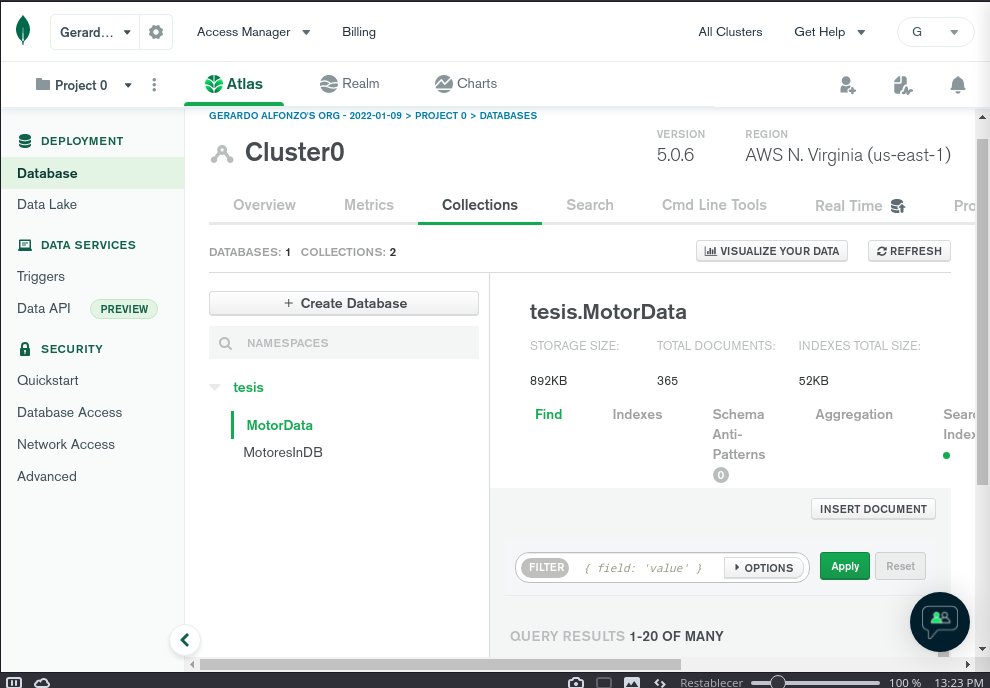
\includegraphics[width=\linewidth]{servers/clusterBBDD.png}
        Base de datos implementada en MongoDB Atlas.    \label{img:clusterBBDD}
	\end{figure}

\subsection{LLENADO DE LA BASE DE DATOS}
    Para el llenado con la información se desarrolló un Script en Golang,
    llamado ``LlenarBBDD"\ , que
    se encarga de hacer las peticiones al modelo y a la base de datos de forma
    automática, realiza 120 peticiones, equivalentes a 120 días, con un aumento
    progresivo del nivel de daño cada 40 días-peticiones. Al ser un Script funciona
    mediante la terminal y utiliza las banderas expuestas en la tabla
    \ref{tab:BanderasLLenadoBBDD} para tomar la información. La utilizacion del
    mismo puede verse en \ref{img:scriptBBDD}

\begin{table}[ht]
        \begin{center}
        \caption[Banderas Script para el llenado de la BBDD]{
        Banderas utilizables al momento de llamar el Script para llenar la información
        de la base de datos}
        \label{tab:BanderasLLenadoBBDD}

            \vspace{0.3cm}
            \begin{tabular}{|c|p{7cm}|p{5cm}|}
                \hline
                Bandera & Descripción & Requerimiento \\\hline
                -i & Para especificar el Id del Motor. & Requerida.\\\hline
                -d & Para indicar el nivel de daño  & Opcional, por defecto 1.\\\hline
                -c & Indicar las características e información del motor & Opcional, por defecto ``Estado del motor".\\\hline
                -s1& Especificar el Id del sensor 1 &Requerida.\\\hline
                -s2& Especificar el Id del sensor 2 &Requerida.\\\hline
                -s3& Especificar el Id del sensor 3 & Opcional, por defecto se omite.\\\hline
                -s4& Especificar el Id del sensor 4  &Opcional, por defecto se omite.\\\hline
                -r & Reiniciar la base de datos si su valor es ``true"& opcional, por defecto false.\\\hline
                -fi& Fecha de inicio, una cantidad de dias contados hacia atras desde la fecha actual& Opcional, por defecto 90\\\hline
                -ci& Cantidad de interaciones a ejecutarse&Opcional, por defecto, 90
                \\\hline
            \end{tabular}
        \end{center}
    \end{table}

	\begin{figure}[htb]
		\centering
        \caption{Llenado de la BBDD}
        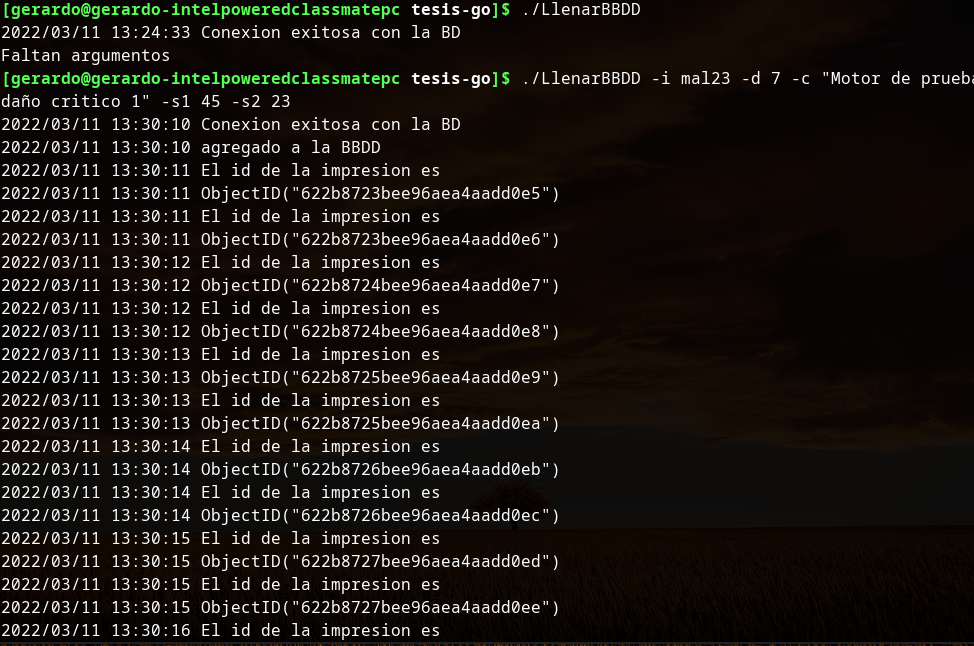
\includegraphics[width=\linewidth]{servers/scriptBBDD.png}
        Llamados al script para llenar la BBDD.    \label{img:scriptBBDD}
	\end{figure}

\subsection{IMPLEMENTACIÓN DE LOS SERVIDORES}

    Los servidores son necesarios para recolectar la información de los sensores,
    establecer una comunicación full dúplex la cual permita obtener información
    a tiempo real del comportamiento del sensor, además de permitir toda la
    interacción Web que da la visibilidad. Dado que estas tareas pueden ser
    separadas y manejadas en forma de API se crearon 2 servidores, permitiendo
    de esta forma la división de la carga de trabajo y, por ende, disminuyendo los
    requerimientos mínimos del equipo en donde se monta cada servidor individual.
    Así mismo, esto permite una mayor escalabilidad y paralelismo, dado que en el
    caso de ser necesaria una ampliación en la capacidad de cómputo se puede colocar
    otro equipo en vez de aumentar las capacidades del equipo ya existente. Este
    hecho permite disminuir los costos sustancialmente.

    La implementación de estos 2 servidores da origen a un \textbf{servidor dedicado
    a sensorica}, desarrollado como un micro-servicio en el lenguaje de programación
    Go (también conocido como Golang) por las razones previamente expuestas, y
    a un \textbf{servidor dedicado al tratamiento Web} desarrollado con una
    combinación de Python y el Framework Django para el Backend y HTML-CSS-JavaScript
    con el Framework de React en un paradigma multipaginas de renderizado desde
    el servidor para el frontend-cliente Web.

    \subsubsection{Servidor dedicado a Sensorica}


    Este servidor fue realizado en Go por los motivos expuestos anteriormente y
    cumple la función de micro-servicio, se encarga de la recolección y comunicación
    con la red de sensorica, la cual es implementada por el cliente de la simulación
    y el modelo estadístico, así mismo envía la información relacionada con la
    vista exhaustiva (para esta se requieren mediciones a tiempo real y por esto
    este servidor tiene una conexión full dúplex con los sensores);
    como se observa en la tabla \ref{tab:ServerSensorica}

    Cabe resaltar que ``DireccionIP"\ hace referencia a la dirección en la
    que sera montado (Host) el sitio, en caso de un ambiente local, por
    ejemplo, es ``localhost:8080" (este es el usado para las pruebas,
    cuando se cambia a producción se modifica por el del Host contratado)

    \begin{table}[ht]
        \begin{center}
        \caption[Funciones Servidor Sensorica]{ Relación de punto de acceso y
        funcionalidad implementada en el servidor de sensorica}
        \label{tab:ServerSensorica}

            \vspace{0.3cm}
            \begin{tabular}{|p{5cm}|p{10cm}|}
                \hline
                Dirección       & Tarea realizada
                \\\hline\hline
                DireccionIP/sensormessage &
                Se encarga del comportamiento, acceso
                e intercambio de información sensor-servidor. Es una comunicación
                bidireccional con Http2 (Https) y se intercambian por el canal
                establecido tanto la información de medición diaria, (después es
                subida a la base de datos) como la
                información de medición exhaustiva (es enviada al cliente que
                la solicitó).

                \\\hline
                DireccionIP/exhaustive \textbf{?idMotor=identificador}   &
                Se encarga de solicitar la información para la vista exhaustiva,
                el identificador único del motor que se solicita la data
                es enviado por el Url (?idMotor=identificador) .
                \\\hline
            \end{tabular}
        \end{center}
    \end{table}


    El primer ``Endpoint"\ (DireccionIP/sensormessage) realiza las siguientes tareas:

    \begin{itemize}
        \item Establecer una conexión Http2 con los solicitantes; para esto se intercambian,
            además de los paquetes e información necesarios para establecer el protocolo,
            unos mensajes que permiten identificar el motor y la cadena de sensores
            correspondientes a esta información.
            %
        \item Posteriormente, se revisa si el motor
            tiene una conexión activa (no debe  existir por unicidad de la información)
            y si ya se ha recibido información de este motor previamente; de no ser así,
            se agrega a la lista de motores de la que se posee información.
            %
        \item En este punto el servidor se dedica a escuchar la llegada o solicitud
            de información. Esta puede ser del sensor con el que se estableció
            conexión (mediante un canal interno) o  de la solicitud de información
            para una vista exhaustiva. Para cada caso se hace lo siguiente:
            \begin{itemize}
                \item[*] Si es información, se verifica que venga en formado válido
                    y se sube a la base de datos.
                \item[*] Si es una solicitud de información, se verifica que
                    la conexión con el motor sea la indicada y se solicita la
                    información, se espera la respuesta y se envía por el mismo
                    canal interno. Esta solicitud es hecha por el segundo Endpoint.
                \item[*] No se dio ninguno de los casos, entonces el cliente se
                    desconecta. Se procede a eliminar la conexión y la lista,
                    mediante un procedimiento de cierre de conexión.
            \end{itemize}
            %
        \item Finalmente, existe un procedimiento de cierre de conexión ya sea
            por solicitud del cliente o por un error ocurrido.
    \end{itemize}


    El segundo ``Endpoint"\ (DireccionIP/exhaustive\textbf{?idMotor=identificador})
    realiza las siguientes tareas:

    \begin{itemize}
        \item Decodifica el URL enviado para obtener el parámetro (idMotor) y
            comprueba su existencia. En caso de error se envía un mensaje
            de petición incorrecta.
            %
        \item Se comprueba que el motor solicitado exista en las conexiones
            actuales. Es importante resaltar que se refiere a la conexión
            bidireccional, ya que de caso contrario no se puede obtener información
            a tiempo real. Por esto, si la conexión es inexistente, se envía un
            mensaje de petición incorrecta, no se puede conectar al motor.
            %
        \item Se solicita por un canal interno al otro Endpoint la información
            deseada y se espera su respuesta.
            %
        \item Se envía la respuesta con estado de creado y la información.
    \end{itemize}

    El servidor corriento es simplemente una terminal ejecutando un programa,
    puede ser visto en la imagen \ref{img:serverSensoricaRunning}.

	\begin{figure}[htb]
		\centering
        \caption{Servidor de sensorica}
        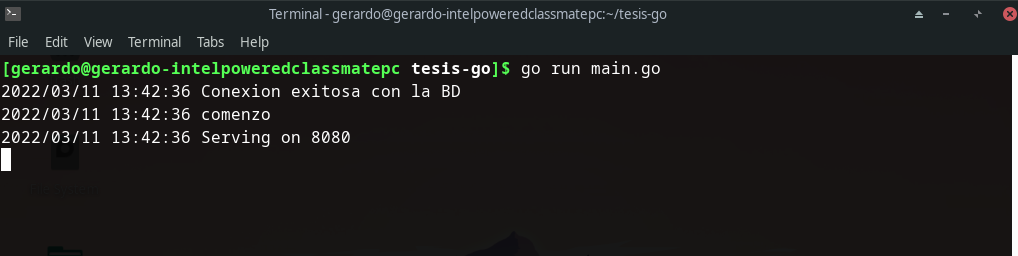
\includegraphics[width=\linewidth]{servers/serverSensoricaRunning.png}
        Inicio de ejecucion del servidor de sensorica.    \label{img:serverSensoricaRunning}
	\end{figure}

    \subsubsection{Servidor Web}
    Este servidor fue realizado en Python con el Framework Django
    por los motivos expuestos anteriormente y cumple la función de servidor Web,
    es el servidor principal ya que se encarga de enviar y solicitar información
    para crear la visualización del cliente, además de estudiar y crear las gráficas
    y enviar información al cliente Web para análisis.
    Sus conexiones son por el protocolo Http, y Https para la petición de información
    exhaustiva con el microservicio de sensorica. y realiza las tareas expuestas
    en la tabla \ref{tab:serWeb}

    Cabe resaltar que ``DireccionIP"\ hace referencia a la dirección en la
    que será montado (Host) el sitio, en caso de un ambiente local, por
    ejemplo, es ``localhost:8000" (este es el usado para las pruebas,
    cuando se cambia a producción se modifica por el del Host contratado)

    \begin{table}[ht]
        \begin{center}
        \caption[Funciones Servidor Web]{ Relación de punto de acceso y
        funcionalidad implementada en el servidor Web }
        \label{tab:serWeb}

            \vspace{0.3cm}
            \begin{tabular}{|p{5cm}|p{10cm}|}
                \hline
                Dirección       & Tarea realizada
                \\\hline\hline
                DireccionIP/ &
                Enviar el HTML necesario, mediante un Template de Django,
                para mostrar la vista general en el navegador.
                \\\hline
                DireccionIP/especifica \textbf{?IdMotor=identificador}&
                Enviar el HTML necesario, mediante un Template de Django,
                para mostrar la vista especifica en el navegador.
                \\\hline
                DireccionIP/exhaustiva \textbf{?IdMotor=identificador}  &
                Enviar el HTML necesario, mediante un Template de Django,
                para mostrar la vista exhaustiva en el navegador.
                \\\hline
                DireccionIP/ static/... &
                Es una funcionalidad del servidor la cual permite el envío de
                archivos estáticos por solicitudes externas, ya sea por un
                requerimiento del HTML o del JavaScript.
                \\\hline
                DireccionIP/ get\_data\_motores &
                API que entrega  una lista, formato JSON,
                con la ultima medición almacenada de cada sensor en la base de
                datos.
                \\\hline
                DireccionIP/ get\_list\_motores &
                API que entrega una lista, formato JSON,
                con todos los motores de los que se
                dispone información en la base de datos.
                \\\hline
                DireccionIP/get\_especifica \textbf{?IdMotor=identificador}&
                API que se encarga de devolver un JSON con toda la información
                en la base de datos referente al motor con el Id pasado en el
                Url, además de las direcciones, en el mismo servidor que serán
                entregadas mediante el Endpoint ``DireccionIP/static/... ", que
                ocupan las gráficas históricas referente a ese motor.
                \\\hline
                DireccionIP/get\_exhaustiva \textbf{?IdMotor=identificador}&
                API que se encarga de devolver un JSON con toda la información
                en la base de datos referente al motor con el Id pasado en el
                Url, además de las direcciones, en el mismo servidor que serán
                entregadas mediante el Endpoint ``DireccionIP/static/... ", que
                ocupan las gráficas históricas y del estudio de Fourier
                referente a ese motor.
                \\\hline
            \end{tabular}

        \end{center}

    \end{table}

    Cada Endpoint realiza las siguientes tareas

    El servidor corriento es simplemente una terminal ejecutando un programa,
    puede ser visto en la imagen \ref{img:serverWebRunning}.

	\begin{figure}[htb]
		\centering
        \caption{Servidor Web}
        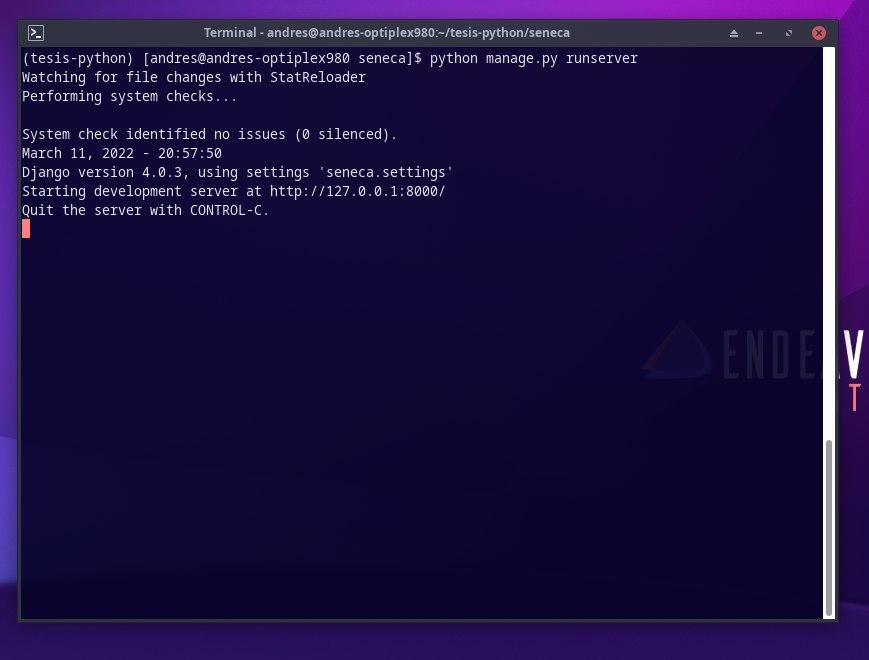
\includegraphics[width=\linewidth]{servers/serverDjangoRunning.png}
        Inicio de ejecucion del servidor Web.    \label{img:serverWebRunning}
	\end{figure}


